\documentclass{standalone}
\usepackage{tikz}
\usetikzlibrary{patterns, positioning}
\usepackage[sfdefault]{ClearSans} %% option 'sfdefault' activates Clear Sans as the default text font
\usepackage[T1]{fontenc}

\begin{document}
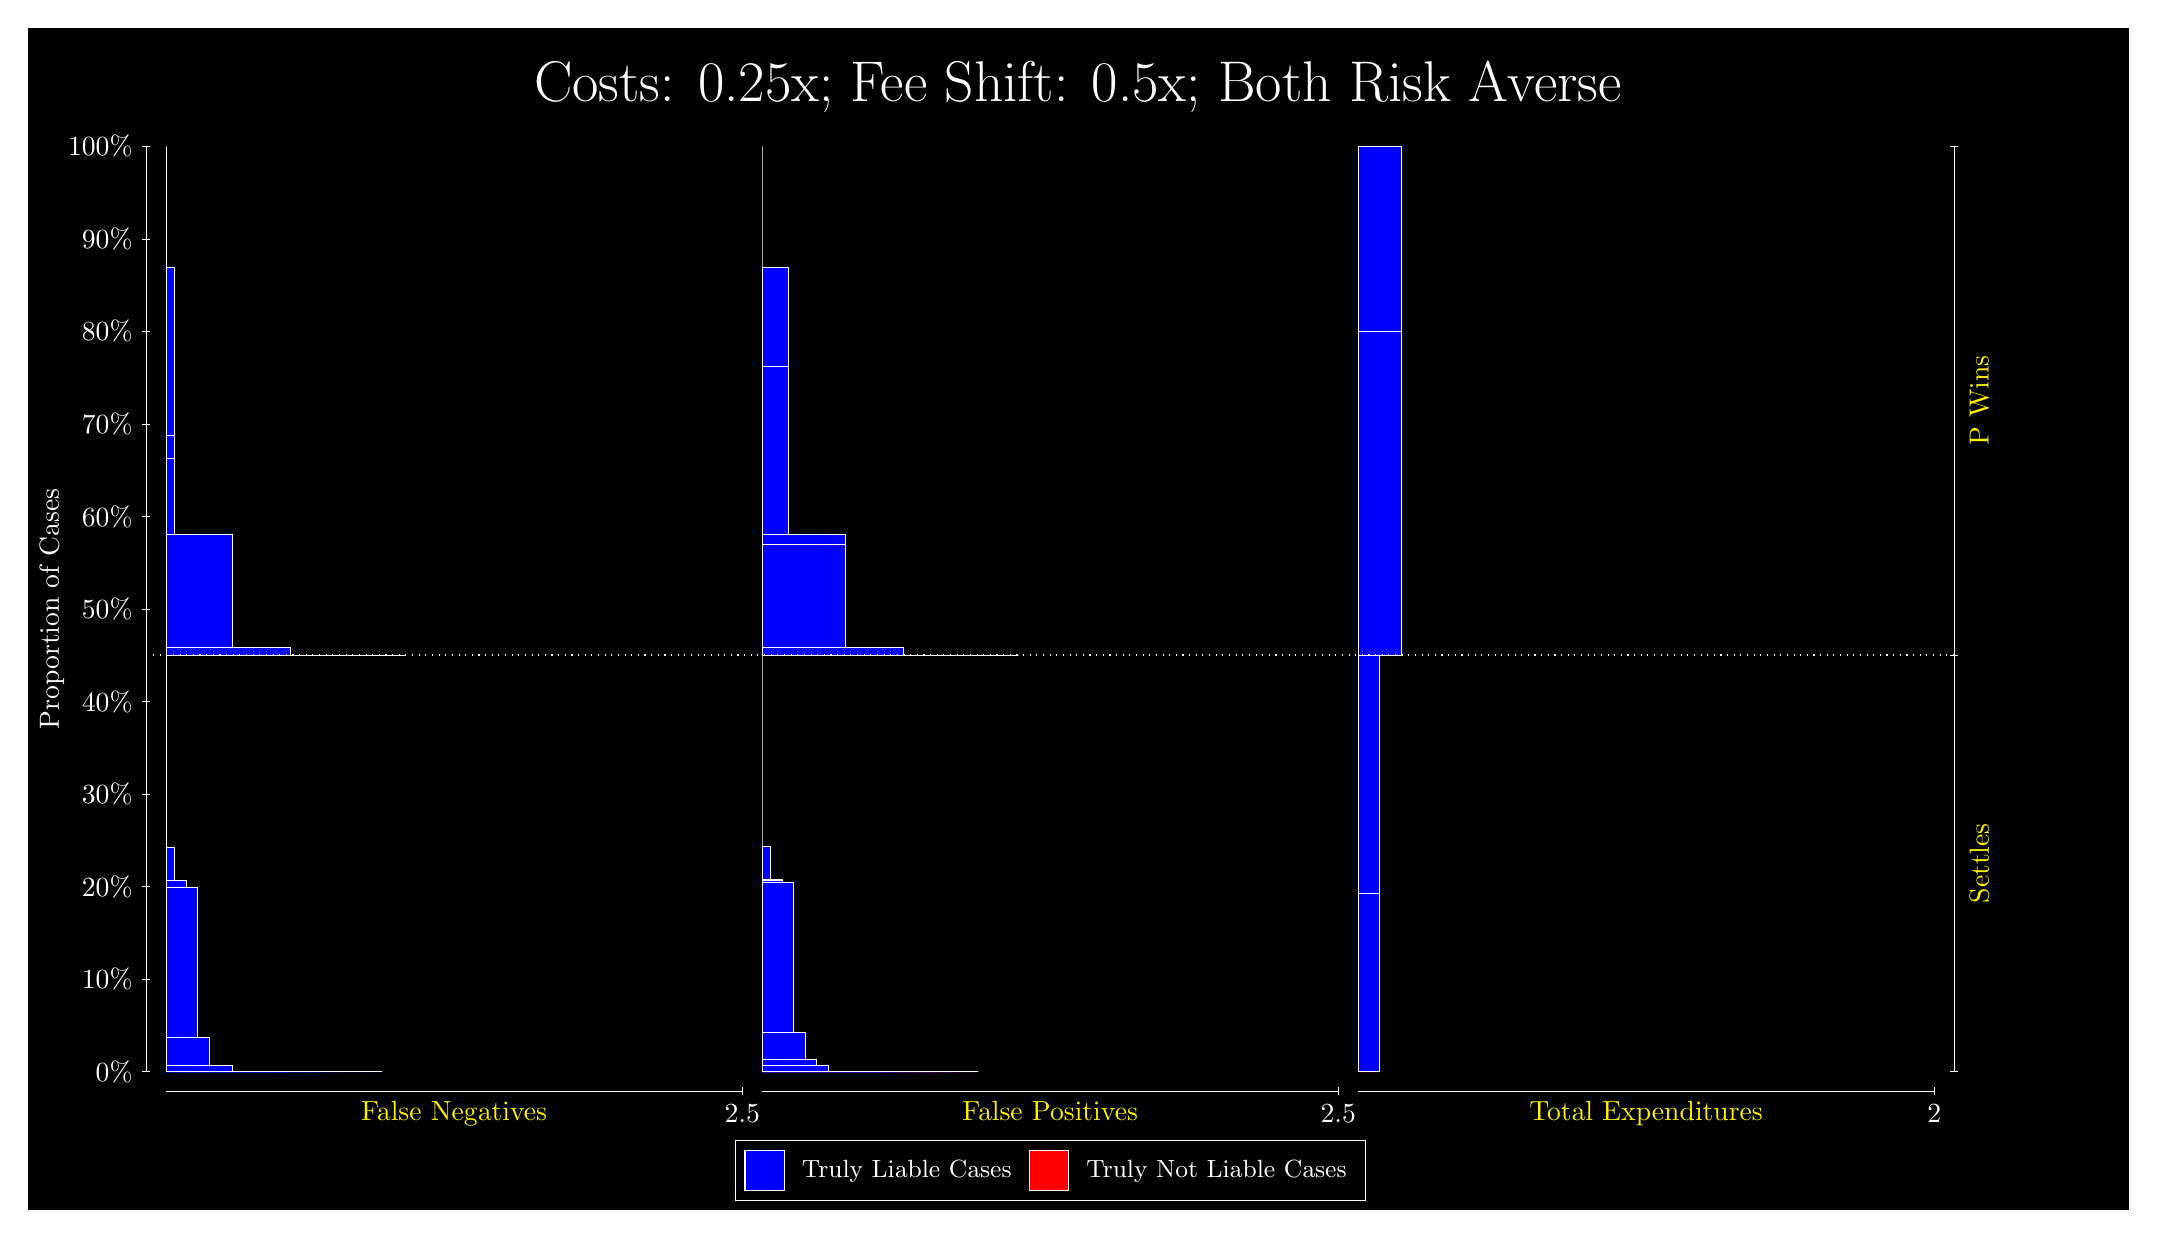
\begin{tikzpicture}
\draw[fill=black] (0,0) rectangle (26.667,15);
\draw[text=white] (0,13.5) rectangle (26.667,15) node[midway] {\huge Costs: 0.25x; Fee Shift: 0.5x; Both Risk Averse};
\draw[white, very thin] (1.5,1.75) -- (1.5,13.5);
\node[rotate=90, text=white, anchor=center] at (0.3, 7.625) {Proportion of Cases};
\draw[white, very thin] (1.45,1.75) -- (1.55,1.75);
\node[text=white, anchor=east] at (1.45, 1.75) {0\%};
\draw[white, very thin] (1.45,2.925) -- (1.55,2.925);
\node[text=white, anchor=east] at (1.45, 2.925) {10\%};
\draw[white, very thin] (1.45,4.1) -- (1.55,4.1);
\node[text=white, anchor=east] at (1.45, 4.1) {20\%};
\draw[white, very thin] (1.45,5.275) -- (1.55,5.275);
\node[text=white, anchor=east] at (1.45, 5.275) {30\%};
\draw[white, very thin] (1.45,6.45) -- (1.55,6.45);
\node[text=white, anchor=east] at (1.45, 6.45) {40\%};
\draw[white, very thin] (1.45,7.625) -- (1.55,7.625);
\node[text=white, anchor=east] at (1.45, 7.625) {50\%};
\draw[white, very thin] (1.45,8.8) -- (1.55,8.8);
\node[text=white, anchor=east] at (1.45, 8.8) {60\%};
\draw[white, very thin] (1.45,9.975) -- (1.55,9.975);
\node[text=white, anchor=east] at (1.45, 9.975) {70\%};
\draw[white, very thin] (1.45,11.15) -- (1.55,11.15);
\node[text=white, anchor=east] at (1.45, 11.15) {80\%};
\draw[white, very thin] (1.45,12.325) -- (1.55,12.325);
\node[text=white, anchor=east] at (1.45, 12.325) {90\%};
\draw[white, very thin] (1.45,13.5) -- (1.55,13.5);
\node[text=white, anchor=east] at (1.45, 13.5) {100\%};

\draw[white, very thin] (24.457,1.75) -- (24.457,13.5);
\draw[white, very thin] (24.407,1.75) -- (24.507,1.75);
\node[anchor=west] at (24.407, 1.75) {};
\draw[white, very thin] (24.407,7.0402) -- (24.507,7.0402);
\node[anchor=west] at (24.407, 7.0402) {};
\draw[white, very thin] (24.407,13.5) -- (24.507,13.5);
\node[anchor=west] at (24.407, 13.5) {};

\draw[white, very thin, fill=blue] (1.75,1.75) rectangle (4.4946,1.75);
\draw[white, very thin, fill=blue] (1.75,1.75) rectangle (3.9091,1.75);
\draw[white, very thin, fill=blue] (1.75,1.75) rectangle (3.7627,1.75);
\draw[white, very thin, fill=blue] (1.75,1.75) rectangle (3.6163,1.75);
\draw[white, very thin, fill=blue] (1.75,1.75) rectangle (3.3236,1.7502);
\draw[white, very thin, fill=blue] (1.75,1.7502) rectangle (3.1772,1.7502);
\draw[white, very thin, fill=blue] (1.75,1.7502) rectangle (3.0308,1.7524);
\draw[white, very thin, fill=blue] (1.75,1.7524) rectangle (2.8844,1.7524);
\draw[white, very thin, fill=blue] (1.75,1.7524) rectangle (2.738,1.7534);
\draw[white, very thin, fill=blue] (1.75,1.7534) rectangle (2.5917,1.8324);
\draw[white, very thin, fill=blue] (1.75,1.8324) rectangle (2.4453,1.8332);
\draw[white, very thin, fill=blue] (1.75,1.8332) rectangle (2.4453,1.834);
\draw[white, very thin, fill=blue] (1.75,1.834) rectangle (2.2989,2.1892);
\draw[white, very thin, fill=blue] (1.75,2.1892) rectangle (2.1525,2.1893);
\draw[white, very thin, fill=blue] (1.75,2.1893) rectangle (2.1525,4.0946);
\draw[white, very thin, fill=blue] (1.75,4.0946) rectangle (2.0062,4.1732);
\draw[white, very thin, fill=blue] (1.75,4.1732) rectangle (1.8598,4.6023);
\draw[white, very thin, fill=red] (1.75,4.6023) rectangle (1.75,4.6023);
\draw[white, very thin, fill=blue] (1.75,4.6023) rectangle (1.75,7.0402);
\draw[white, very thin, fill=blue] (1.75,7.0402) rectangle (4.7873,7.0402);
\draw[white, very thin, fill=blue] (1.75,7.0402) rectangle (4.0554,7.0412);
\draw[white, very thin, fill=blue] (1.75,7.0412) rectangle (3.3236,7.1374);
\draw[white, very thin, fill=blue] (1.75,7.1374) rectangle (2.5917,8.5745);
\draw[white, very thin, fill=blue] (1.75,8.5745) rectangle (1.8598,9.537);
\draw[white, very thin, fill=blue] (1.75,9.537) rectangle (1.8598,9.8303);
\draw[white, very thin, fill=blue] (1.75,9.8303) rectangle (1.8598,11.964);
\draw[white, very thin, fill=red] (1.75,11.964) rectangle (1.75,11.964);
\draw[white, very thin, fill=blue] (1.75,11.964) rectangle (1.75,13.5);
\draw[white, very thin, fill=red] (9.3189,1.75) rectangle (12.063,1.75);
\draw[white, very thin, fill=blue] (9.3189,1.75) rectangle (12.063,1.75);
\draw[white, very thin, fill=red] (9.3189,1.75) rectangle (11.771,1.75);
\draw[white, very thin, fill=blue] (9.3189,1.75) rectangle (11.771,1.75);
\draw[white, very thin, fill=red] (9.3189,1.75) rectangle (11.478,1.75);
\draw[white, very thin, fill=blue] (9.3189,1.75) rectangle (11.478,1.75);
\draw[white, very thin, fill=blue] (9.3189,1.75) rectangle (11.332,1.75);
\draw[white, very thin, fill=blue] (9.3189,1.75) rectangle (11.039,1.75);
\draw[white, very thin, fill=red] (9.3189,1.75) rectangle (10.892,1.75);
\draw[white, very thin, fill=blue] (9.3189,1.75) rectangle (10.892,1.7502);
\draw[white, very thin, fill=blue] (9.3189,1.7502) rectangle (10.746,1.7508);
\draw[white, very thin, fill=blue] (9.3189,1.7508) rectangle (10.6,1.7526);
\draw[white, very thin, fill=red] (9.3189,1.7526) rectangle (10.6,1.7526);
\draw[white, very thin, fill=blue] (9.3189,1.7526) rectangle (10.6,1.7526);
\draw[white, very thin, fill=blue] (9.3189,1.7526) rectangle (10.307,1.7532);
\draw[white, very thin, fill=red] (9.3189,1.7532) rectangle (10.307,1.7532);
\draw[white, very thin, fill=blue] (9.3189,1.7532) rectangle (10.307,1.754);
\draw[white, very thin, fill=blue] (9.3189,1.754) rectangle (10.161,1.833);
\draw[white, very thin, fill=blue] (9.3189,1.833) rectangle (10.014,1.9115);
\draw[white, very thin, fill=blue] (9.3189,1.9115) rectangle (9.8678,2.2521);
\draw[white, very thin, fill=blue] (9.3189,2.2521) rectangle (9.8678,2.2522);
\draw[white, very thin, fill=red] (9.3189,2.2522) rectangle (9.7214,2.2522);
\draw[white, very thin, fill=blue] (9.3189,2.2522) rectangle (9.7214,4.1583);
\draw[white, very thin, fill=blue] (9.3189,4.1583) rectangle (9.575,4.173);
\draw[white, very thin, fill=blue] (9.3189,4.173) rectangle (9.575,4.1879);
\draw[white, very thin, fill=blue] (9.3189,4.1879) rectangle (9.4287,4.617);
\draw[white, very thin, fill=blue] (9.3189,4.617) rectangle (9.3189,7.0402);
\draw[white, very thin, fill=red] (9.3189,7.0402) rectangle (12.576,7.0402);
\draw[white, very thin, fill=blue] (9.3189,7.0402) rectangle (12.576,7.0402);
\draw[white, very thin, fill=red] (9.3189,7.0402) rectangle (11.844,7.0402);
\draw[white, very thin, fill=blue] (9.3189,7.0402) rectangle (11.844,7.0413);
\draw[white, very thin, fill=red] (9.3189,7.0413) rectangle (11.112,7.0413);
\draw[white, very thin, fill=blue] (9.3189,7.0413) rectangle (11.112,7.1389);
\draw[white, very thin, fill=blue] (9.3189,7.1389) rectangle (10.38,8.4399);
\draw[white, very thin, fill=red] (9.3189,8.4399) rectangle (10.38,8.4399);
\draw[white, very thin, fill=blue] (9.3189,8.4399) rectangle (10.38,8.576);
\draw[white, very thin, fill=blue] (9.3189,8.576) rectangle (9.6482,10.71);
\draw[white, very thin, fill=red] (9.3189,10.71) rectangle (9.6482,10.71);
\draw[white, very thin, fill=blue] (9.3189,10.71) rectangle (9.6482,11.966);
\draw[white, very thin, fill=blue] (9.3189,11.966) rectangle (9.3189,13.5);
\draw[white, very thin, fill=red] (16.888,1.75) rectangle (17.162,1.75);
\draw[white, very thin, fill=blue] (16.888,1.75) rectangle (17.162,4.0135);
\draw[white, very thin, fill=red] (16.888,4.0135) rectangle (17.162,4.0135);
\draw[white, very thin, fill=blue] (16.888,4.0135) rectangle (17.162,7.0402);
\draw[white, very thin, fill=red] (16.888,7.0402) rectangle (17.437,7.0402);
\draw[white, very thin, fill=blue] (16.888,7.0402) rectangle (17.437,11.155);
\draw[white, very thin, fill=red] (16.888,11.155) rectangle (17.437,11.155);
\draw[white, very thin, fill=blue] (16.888,11.155) rectangle (17.437,13.5);
\draw[white, dotted] (1.5,7.0402) -- (24.457,7.0402);
\draw[white, very thin] (1.75,1.5) -- (9.0689,1.5);
\node[text=yellow, anchor=north] at (5.4094, 1.5) {False Negatives};
\draw[white, very thin] (9.0689,1.45) -- (9.0689,1.55);
\node[text=white, anchor=north] at (9.0689, 1.45) {2.5};

\draw[white, very thin] (9.3189,1.5) -- (16.638,1.5);
\node[text=yellow, anchor=north] at (12.978, 1.5) {False Positives};
\draw[white, very thin] (16.638,1.45) -- (16.638,1.55);
\node[text=white, anchor=north] at (16.638, 1.45) {2.5};

\draw[white, very thin] (16.888,1.5) -- (24.207,1.5);
\node[text=yellow, anchor=north] at (20.547, 1.5) {Total Expenditures};
\draw[white, very thin] (24.207,1.45) -- (24.207,1.55);
\node[text=white, anchor=north] at (24.207, 1.45) {2};

\node[text=yellow, centered, rotate=90] at (24.777, 4.3951) {Settles};
\node[text=yellow, centered, rotate=90] at (24.777, 10.27) {P Wins};

\draw (12.978300999999998,1.5) node[draw=none] (baseCoordinate) {};
\begin{scope}[align=center]
        \matrix[scale=0.5, draw=white, below=0.5cm of baseCoordinate, nodes={draw}, column sep=0.1cm]{
            \node[rectangle, draw, minimum width=0.5cm, minimum height=0.5cm, fill=blue] {}; &
            \node[draw=none, font=\small, text=white] (B) {Truly Liable Cases}; &
            \node[rectangle, draw, minimum width=0.5cm, minimum height=0.5cm, fill=red] {}; &
            \node[draw=none, font=\small, text=white] (B) {Truly Not Liable Cases}; \\
            };
\end{scope}

\end{tikzpicture}
\end{document}